\documentclass[10pt]{article}
\usepackage{graphicx} % Required for inserting images
\usepackage{amsmath}
\usepackage{amssymb}
\usepackage{parskip}
\usepackage{pgfplots}
\pgfplotsset{width=10cm,height=10cm,compat=1.9}

% We will externalize the figures
% \usepgfplotslibrary{external}
% \tikzexternalize

\usepackage{geometry}
 \geometry{
 a4paper,
 total={170mm,257mm},
 left=20mm,
 top=20mm,
 }

\title{Pre Calculus 12}
\author{Sky Shaver}
\date{April 2026}

\begin{document}

\maketitle

\section{Transformations}


\subsection{Functions and Their Graphs}


\textbf{Relations:}
\begin{itemize}
    \item A relation R is a set of ordered pairs
    \item The domain of R is the set of first coordinates of the ordered pairs
    \item the range R is the set of second coordinates of the ordered pairs
\end{itemize}
A relation can be represented in different ways:
\begin{itemize}
    \item a set of ordered pairs
    \item a table of values
    \item a graph
    \item an equation
\end{itemize}


y is equal to the \(\sqrt{x}\) where x is all integers that are perfect squares between (0, 16) \\
\begin{tabular}{|c|c|}
    \hline
    x     & y      \\
    \hline
    y = 0 & x = 0  \\
    y = 1 & x = 1  \\
    y = 2 & x = 4  \\
    y = 3 & x = 9  \\
    y = 4 & x = 16 \\
    \hline
\end{tabular}


for: \(y = 2x + 1 \) \\
Domain = [0, -2, -4, 2, 4] \\
Range = [1, -3, -7, 5, 9]


\textbf{What is the purpose of joining the points with a line?} \\
- joining the points shows the relations include more ordered pairs not just the ones for this set of values


\textbf{Conventions:} \\
- no endpoints means no termination for graph \\
- open dot means approaches and gets infinitely close \\
- always read inequalities from the variable to the number \(x \leq 7\) or \(7 \leq x\) is "x is greater than or equal to 7"


\textbf{Relation as expressed by x,y graph:} \\
Domain: set of x values represented by the graph \\
- always start at left most point and trace to right most point \\
- \(-6 < x \leq 7\) (here -6 is an open dot and 7 is a closed dot so we can get to 7 but we can never get to -6) \\
Range: set of y values represented by the graph \\
- can start at max or min \\
-  \(- 4 \leq y < 7\) \\
Domain: \(-3 \leq x \leq 8\) \\
Range: \(-2 \leq y \leq 8\)


\textbf{What do functions do?} \\
- for every possible input value there is one output value \\
- a function is a special kind of relation \\
- there is a difference between functions and relations


\textbf{Defintion of a function:} \\
- a function is a relation which assigns to each element in the domain(x) at single element in the range(y) \\
- for every value of the domain there is one and only one value of the range \\
- if two points can be joined by a vertical line then the graph is not a function

\textbf{Is an equation a function?} \\
- if an x value can be found that produces more than one value of y then the equation is not a function \\
- \(y = x^2\) (if an equation is solved for y it is a function) \\
- \(y^2 = x\) (here to simplify for y we get \(y = +/- \sqrt{x}\) so there are two values of y for x (\(x = 4 \therefore \) \(y = 2 \And y = -2\))) \\
- if \(y^2\) or if \(x = \mathbb{R} \)  it's not a function

% https://www.overleaf.com/learn/latex/Pgfplots_package#Reference_guide
% https://shantoroy.com/latex/how-to-draw-line-graph-using-pgfplots-latex/
\begin{tikzpicture}
    \begin{axis} [
            title={sample x y graph},
            xlabel={X},
            ylabel={Y},
            xmin=-10, xmax=10,
            ymin=-10, ymax=10,
            xtick={-10, -5, 0, 5, 10},
            ytick={-10, -5, 0, 5, 10},
            legend pos=north west,
            ymajorgrids=true,
            grid style=dashed,
        ]

        % [grid=both,
        %      % number of ticks in between grids, 9 ticks = 10 cells
        %      minor tick num=9,
        %      % define regular grid style with line width and color
        %      grid style={line width=.2pt, draw=black!10},
        %      % define major grid style with line width and color
        %      major grid style={line width=.4pt,draw=black!50},
        %      axis lines=middle,
        %      enlargelimits={abs=0.1},
        %      % define width and height
        %      width=12cm, height=9cm
        %     ]

        \addplot[
            color=blue,
            mark=oplus*, % oplus* is a filled circle, o is an empty circle
        ]
        coordinates {
                (-3, -4) (-2, 5) (0, -9) (1, 8) (2, 8) (3, 9) (4, 6)
            };
        % \legend{CuSO\(_4\cdot\)5H\(_2\)O}

    \end{axis}
\end{tikzpicture}


\textbf{X + Y Intercept}: \\
\(2y+3x = -6\) \\
- to find \(y\) intercept make \(x = 0\) in function \(\therefore y = -3 \) \\
\hspace*{1em} \(2y + 3(0) = -6\) \\
\hspace*{1em} \(\frac{y}{2} = \frac{-6}{2}\) \\
\hspace*{1em} \(y = -3\) \\
- to find \(x\) intercept make \(y = 0\) in function \(\therefore x = -2 \) \\
\hspace*{1em} \(2(0) + 3x = -6\) \\
\hspace*{1em} \(\frac{3x}{3} = \frac{-6}{3}  \) \\
\hspace*{1em} \(x = -2\)


\textbf{Slope Intercept Form}: \\
\(y = mx + b\) \\
slope = \( \frac{rise}{run}\) \\
only rise or run can be -ve \\
\hspace*{1em} \(2y = -6 -3x\) \\
\hspace*{1em} \(y = \frac{-6-3x}{2}\) \\
\hspace*{1em} \(y = \frac{-3}{2}x - 3\)


\textbf{The Constant Function}: \\
\(y = 1\) \\
\(y = mx + b\) aka The Slope Intercept form \\
The domain for a constant \(f\) is all \(\mathbb{R} \) \\
The range is a single \(\mathbb{R} \) like 1
\clearpage
\textbf{The Quadratic Function}: \\
\(y = x^2 \) \\
\begin{tabular}{|c|c|}
    \hline
    x      & y     \\
    \hline
    x = 3  & y = 9 \\
    x = 2  & y = 4 \\
    x = 1  & y = 1 \\
    x = 0  & y = 0 \\
    x = -1 & y = 1 \\
    x = -2 & y = 4 \\
    x = -3 & y = 9 \\
    \hline
\end{tabular}


\begin{tikzpicture}
    \begin{axis} [
            title={quadratic function},
            xlabel={X},
            ylabel={Y},
            xmin=-10, xmax=10,
            ymin=-10, ymax=10,
            xtick={-10, -5, 0, 5, 10},
            ytick={-10, -5, 0, 5, 10},
            ymajorgrids=true,
            xmajorgrids=true,
            grid style=dashed,
        ]

        \addplot[
            domain=-3:3,
            samples=100,
            color=blue
        ]
        { x^2 };
        % \legend{CuSO\(_4\cdot\)5H\(_2\)O}

    \end{axis}
\end{tikzpicture}

\(D: x \in \mathbb{R}\) \\
\(R: y \geq 0 \) \\
- every parabola has an axis of symettry where \( x = 0 \) \\
- every vertical line the equation will always be x = "where the line crosses 0"
\clearpage

\textbf{Linear Function}: \\
\(y = x\) \\
\(y = -3x + 1\) \\
\(D: x \in \mathbb{R}\) \\
\(R: y \in \mathbb{R}\) \\
\begin{tikzpicture}
    \begin{axis} [
            title={linear function},
            xlabel={X},
            ylabel={Y},
            xmin=-10, xmax=10,
            ymin=-10, ymax=10,
            xtick={-10, -5, 0, 5, 10},
            ytick={-10, -5, 0, 5, 10},
            ymajorgrids=true,
            xmajorgrids=true,
            grid style=dashed,
        ]

        \addplot [
            domain=-10:10,
            samples=100,
            color=blue
        ]
        { -3*x+1 };
        % \legend{CuSO\(_4\cdot\)5H\(_2\)O}

    \end{axis}
\end{tikzpicture}


\textbf{Cubic Function}: \\
\(y = x^3\) \\
\(D: x \in \mathbb{R}\) \\
\(R: y \in \mathbb{R}\) \\
- results in an S shaped curve \\
\begin{tikzpicture}
    \begin{axis} [
            title={cubic function},
            xlabel={X},
            ylabel={Y},
            xmin=-10, xmax=10,
            ymin=-10, ymax=10,
            xtick={-10, -5, 0, 5, 10},
            ytick={-10, -5, 0, 5, 10},
            ymajorgrids=true,
            xmajorgrids=true,
            grid style=dashed,
        ]

        \addplot [
            domain=-3:3,
            samples=100,
            color=blue
        ]
        { x^3 };
        % \legend{CuSO\(_4\cdot\)5H\(_2\)O}

    \end{axis}
\end{tikzpicture}


\clearpage

\textbf{Reciprocal Function}: \\
\(y = \frac{1}{x}\) \\
\(D: x \neq 0 \And x \in \mathbb{R}\) \\
\(R: y \neq 0 \And y \in \mathbb{R}\) \\
- Asymptote: is a line where the graph will approach the line infinitely but never touch the line


\begin{tikzpicture}
    \begin{axis} [
            title={reciprocal function},
            xlabel={X},
            ylabel={Y},
            xmin=-10, xmax=10,
            ymin=-10, ymax=10,
            xtick={-10, -5, 0, 5, 10},
            ytick={-10, -5, 0, 5, 10},
            ymajorgrids=true,
            xmajorgrids=true,
            grid style=dashed,
        ]

        \addplot [
            domain=-10:10,
            samples=100,
            color=blue
        ]
        { 1/x };
        % \legend{CuSO\(_4\cdot\)5H\(_2\)O}

    \end{axis}
\end{tikzpicture}

\textbf{Absolute Function}: \\
\(y = \left| x \right| \) \\
\(D: x \in \mathbb{R}\) \\
\(R: y \geq 0 \)


\begin{tikzpicture}
    \begin{axis} [
            title={absolute function},
            xlabel={X},
            ylabel={Y},
            xmin=-10, xmax=10,
            ymin=-10, ymax=10,
            xtick={-10, -5, 0, 5, 10},
            ytick={-10, -5, 0, 5, 10},
            ymajorgrids=true,
            xmajorgrids=true,
            grid style=dashed,
        ]

        \addplot [
            domain=-10:10,
            samples=100,
            color=blue
        ]
        { abs(x) };
        % \legend{CuSO\(_4\cdot\)5H\(_2\)O}

    \end{axis}
\end{tikzpicture}
\clearpage

\textbf{Semi Circle Function}: \\
\(y = \sqrt{16-x^2} \) \\
\(D: -4 \leq  x \leq 4 \) \\
\(R: 0 \leq y \leq 4 \) \\
- \(\sqrt{16}\) gives us the domain and the range


\begin{tikzpicture}
    \begin{axis} [
            title={semi circle function},
            xlabel={X},
            ylabel={Y},
            xmin=-10, xmax=10,
            ymin=-10, ymax=10,
            xtick={-10, -5, 0, 5, 10},
            ytick={-10, -5, 0, 5, 10},
            ymajorgrids=true,
            xmajorgrids=true,
            grid style=dashed,
        ]

        \addplot [
            domain=-10:10,
            samples=100,
            color=blue
        ]
        { sqrt(16-x^2) };
        % \legend{CuSO\(_4\cdot\)5H\(_2\)O}

    \end{axis}
\end{tikzpicture}
\clearpage


\subsection{Translating Graphs of Functions}


\textbf{Comparing \(y = x^2\) to \(y = (x-7)^2\)}: \\
- replacing x with x - h
- moves the graph by a translation (7 units to the right)


\begin{tikzpicture}
    \begin{axis} [
            title={Comparison Plot},
            xlabel={X},
            ylabel={Y},
            xmin=-10, xmax=10,
            ymin=-10, ymax=10,
            xtick={-10, -5, 0, 5, 10},
            ytick={-10, -5, 0, 5, 10},
            ymajorgrids=true,
            xmajorgrids=true,
            grid style=dashed,
        ]

        \addplot [
            domain=-10:10,
            samples=100,
            color=blue
        ]
        { x^2 };
        \addplot [
            domain=-10:10,
            samples=100,
            color=red
        ]
        { (x-7)^2 };


    \end{axis}
\end{tikzpicture}


\textbf{Comparing \(y = x^2\) to \(y = (x+5)^2\)}: \\
- replacing x with x - h \\
- moves the graph by a translation (5 units to the left)


\begin{tikzpicture}
    \begin{axis} [
            title={Comparison Plot},
            xlabel={X},
            ylabel={Y},
            xmin=-10, xmax=10,
            ymin=-10, ymax=10,
            xtick={-10, -5, 0, 5, 10},
            ytick={-10, -5, 0, 5, 10},
            ymajorgrids=true,
            xmajorgrids=true,
            grid style=dashed,
        ]

        \addplot [
            domain=-10:10,
            samples=100,
            color=blue
        ]
        { x^2 };
        \addplot [
            domain=-10:10,
            samples=100,
            color=red
        ]
        { (x+5)^2 };


    \end{axis}
\end{tikzpicture}

\textbf{Comparing \(y = f(x)\) to \(y = f(x-h)\)}: \\
- so \(y = x^2\) becomes \(y = (x - h)^2\) \\
- \(h\) refers to horizontal translation \\
- if \(h > 0\) then the graph is translated \(h\) units to the right \\
- if \(h < 0\) then the graph is translated \(h\) units to the left \\
- if function is absolute ie \(y = \left| x \right| \) \\
- \(y = \left| x - 5\right|\) translates the graph 5 units to the right \\
- in this case \(h = 5\) \\
- if \(h\) is +ve like \(y = \left| x + 3\right|\) then translate 3 units to the left \\
- in this case \(h = -3\)

- write the new equation for each translation on the function \(y = \sqrt{x}\) \\
a) a horizontal translation of 5 units left \\
- \(y = \sqrt{x+5} \therefore h = -5\) \\
b) a horizontal translation of 3 units right \\
- \(y = \sqrt{x - 3} \therefore h = 3\)


\textbf{Comparing \(y = \left|x\right|\) to \(y - 3 = \left|x\right|\)}: \\
- replacing \(y\) with \(y - k\) \\
- \(k\) is vertical translation \\
- \(k = 3\) and the graph is translated 3 units up vertically \\
- \(y - 3 = \left|x\right|\) is equal to \(y = \left|x\right| + 3\)


\begin{tikzpicture}
    \begin{axis} [
            title={Comparison Plot},
            xlabel={X},
            ylabel={Y},
            xmin=-10, xmax=10,
            ymin=-10, ymax=10,
            xtick={-10, -5, 0, 5, 10},
            ytick={-10, -5, 0, 5, 10},
            ymajorgrids=true,
            xmajorgrids=true,
            grid style=dashed,
        ]

        \addplot [
            domain=-10:10,
            samples=100,
            color=blue
        ]
        { abs(x) };
        \addplot [
            domain=-10:10,
            samples=100,
            color=red
        ]
        { abs(x)+3 };


    \end{axis}
\end{tikzpicture}


\textbf{Comparing \(y = \left|x\right|\) to \(y + 7 = \left|x\right|\)}: \\
- replacing \(y\) with \(y - k\) \\
- \(k\) is vertical translation \\
- \(k = -7\) and the graph is translated 7 units down vertically \\
- \(y + 7 = \left|x\right|\) is equal to \(y = \left|x\right| - 7\)


\begin{tikzpicture}
    \begin{axis} [
            title={Comparison Plot},
            xlabel={X},
            ylabel={Y},
            xmin=-10, xmax=10,
            ymin=-10, ymax=10,
            xtick={-10, -5, 0, 5, 10},
            ytick={-10, -5, 0, 5, 10},
            ymajorgrids=true,
            xmajorgrids=true,
            grid style=dashed,
        ]

        \addplot [
            domain=-10:10,
            samples=100,
            color=blue
        ]
        { abs(x) };
        \addplot [
            domain=-10:10,
            samples=100,
            color=red
        ]
        { abs(x)-7 };


    \end{axis}
\end{tikzpicture}

\clearpage
\textbf{Comparing \(y = f(x)\) to \(y + k = f(x)\)}: \\
- \(k\) refers to vertical translation \\
- if \(k < 0\) then the graph is translated \(k\) units up \\
- if \(k > 0\) then the graph is translated \(k\) units down


\textbf{Example 01:}
- Sketch the graph of the function \(y=\sqrt{x+3}-4\) \\
a) What is the domain and the range of this new function \\
D: \(x \geq -3\) \\
R: \(y \geq -4\) \\
b) what are the x and y intercepts? \\
X intercept: \\
\hspace*{1em} \(y=0\) \\
\hspace*{1em} \(0 = \sqrt{x+3}-4\) \\
\hspace*{1em} \(4=\sqrt{x+3}\) \\
\hspace*{1em} \(4^2=(\sqrt{x+3})^2\) \\
\hspace*{1em} \(16=x+3\) \\
\hspace*{1em} \(x=13\) \\
Y intercept: \\
\hspace*{1em} \(x=0\) \\
\hspace*{1em} \(y = \sqrt{0+3}-4\) \\
\hspace*{1em} \(y=\sqrt{3}-4\)


\textbf{Example 02:}
- Sketch the graph of the function \(y = (x-4)^2 + 1 \) \\
a) What is the domain and the range of this function? \\
D: \(x = \mathbb{R} \) \\
D: \(y \geq 1 \) \\
b) what are the x and y intercepts? \\
X intercept: \\
\hspace*{1em} \(y=0\) \\
\hspace*{1em} \(0 = (x-4)^2 + 1\) \\
\hspace*{1em} \(-1 = (x-4)^2\) \\
- we cannot do \(\sqrt{-1} \therefore\) no x intercept \\
Y intercept: \\
\hspace*{1em} \(x=0\) \\
\hspace*{1em} \(y = (0-4)^2 + 1\) \\
\hspace*{1em} \(y = (-4)^2 + 1\) \\
\hspace*{1em} \(y = 16 + 1\) \\
\hspace*{1em} \(y = 17\)


\textbf{Example 03:} \\
- Sketch the graph of the function \(y = \sqrt{16 - (x-3)^2} \) \\
a) What is the domain and the range of this function? \\
\(D: -1 \leq  x \leq 7 \) this is a translation the -3 becomes the h value 3 so offset by +3\\
\(R: 0 \leq y \leq 4 \)


\textbf{Example 04:} \\
- Given the graph of the function \(y = f(x)\) sketch the graph \(y = f(x+3) -2\)  \\
- graph is translated 3 units to the left \(x+3\) \\
- graph is tranlated 2 units down \(-2\)


\textbf{Example 05:} \\
- Given the point \((3, -4)\) determine the new coordinates of the translated image \(y = f(x+4) +2\)  \\
- translate 4 to the left (-4) \\
- translate 2 up, (+2) \\
- \((-1, -2)\)
\clearpage


\textbf{Formative Assessment:}


1) Given the graph of the function \(y = f(x)\) sketch the graph \(y + 4 = f(x+3)\)  \\
\hspace*{1em} \(y = f(x+3) - 4\) \\
\hspace*{1em} translate 3 units to the left and 4 units down


2) Write the equation of the image of  \(y = f(x)\) after each transformation  \\
\hspace*{1em} a) a horizontal translation of 9 units left \\
\hspace*{2em} \(y = f(x + 9)\)\\
\hspace*{1em} b) A vertical translation of 3 units up \\
\hspace*{2em} \(y = f(x) + 3\)\\
\hspace*{1em} c) A horizontal translation of 1 unit left and 7 units down \\
\hspace*{2em} \(y = f(x + 1) - 7\)


3) What happens to the graph of the function \(y = f(x)\) if you make the following changes \\
\hspace*{1em} a) replace \(x\) with \(x - 6\) \\
\hspace*{2em} translate 6 units to the right\\
\hspace*{1em} b) replace \(y\) with \(y + 4\) \\
\hspace*{2em} translate 4 units down\\
\hspace*{1em} c) replace \(x\) with \(x + 2\) and \(y\) with \(y-5\)\ \\
\hspace*{2em} translate 2 units to the left and 5 units up


4) Sketch the graphs of the function on the same grid \\
\hspace*{1em} a) \(y = x^2\) \\
\hspace*{1em} b) \(y = (x+4)^2\) \\
\hspace*{1em} c) \(y = (x-3)^2 - 8\) \\
\hspace*{2em} these are all parabolic functions with translations


\begin{tikzpicture}
    \begin{axis} [
            title={Comparison Plot},
            xlabel={X},
            ylabel={Y},
            xmin=-10, xmax=10,
            ymin=-10, ymax=10,
            xtick={-10, -5, 0, 5, 10},
            ytick={-10, -5, 0, 5, 10},
            ymajorgrids=true,
            xmajorgrids=true,
            grid style=dashed,
        ]

        \addplot [
            domain=-10:10,
            samples=100,
            color=blue
        ]
        { x^2 };

        \addplot [
            domain=-10:10,
            samples=100,
            color=red
        ]
        { (x+4)^2 };

        \addplot [
            domain=-10:10,
            samples=100,
            color=green
        ]
        { (x-3)^2-8 };


    \end{axis}
\end{tikzpicture}


5) The function \(y = f(x)\) is to tranformed to \(y = f(x - c) + d\) determine the value of c and d for each \\
\hspace*{1em} \textbf{TAKE NOTE OF THE - BEFORE C WHEN SOLVING THIS, LEFT IS \(y = f(x + 3)\) BUT IT BECOMES -3 TO GET -(-3) or +3} \\
\hspace*{1em} a) 3 units left \(\therefore c = -3 \And d = 0\)\\
\hspace*{1em} b) 2 units down \(\therefore c = 0 \And d = -2\) \\
\hspace*{1em} c) 6 units right and 9 units down  \(\therefore c = +6 \And d = -9\)
\clearpage


6) Sketch the graphs of the function on the same grid \\
\hspace*{1em} a) \(y = \sqrt{4-x^2}\) \\
\hspace*{1em} b) \(y = \sqrt{4-(x+6)^2}\) \\
\hspace*{2em} translated 6 units to the left \\
\hspace*{1em} c) \(y = \sqrt{4-(x-2)^2}-7\) \\
\hspace*{2em} translated 2 units to the right and 7 units down \\
\hspace*{1em} These are all semi circle functions with translations


\begin{tikzpicture}
    \begin{axis} [
            title={Comparison Plot},
            xlabel={X},
            ylabel={Y},
            xmin=-10, xmax=10,
            ymin=-10, ymax=10,
            xtick={-10, -5, 0, 5, 10},
            ytick={-10, -5, 0, 5, 10},
            ymajorgrids=true,
            xmajorgrids=true,
            grid style=dashed,
        ]

        \addplot [
            domain=-10:10,
            samples=100,
            color=blue
        ]
        { sqrt(4-x^2) };

        \addplot [
            domain=-10:10,
            samples=100,
            color=red
        ]
        { sqrt(4-(x+6)^2) };

        \addplot [
            domain=-10:10,
            samples=100,
            color=green
        ]
        { sqrt(4-(x-2)^2) - 7 };


    \end{axis}
\end{tikzpicture}


7) Sketch the graphs of the function on the same grid \\
\hspace*{1em} a) \(y = \frac{1}{x}\) \\
\hspace*{1em} b) \(y = \frac{1}{x-7}\) \\
\hspace*{2em} translated 7 units to the right \\
\hspace*{1em} c) \(y = \frac{1}{x+5} + 4\) \\
\hspace*{2em} translated 5 units to the left and 4 units up \\
\hspace*{1em} These are all reciprocal functions with translations


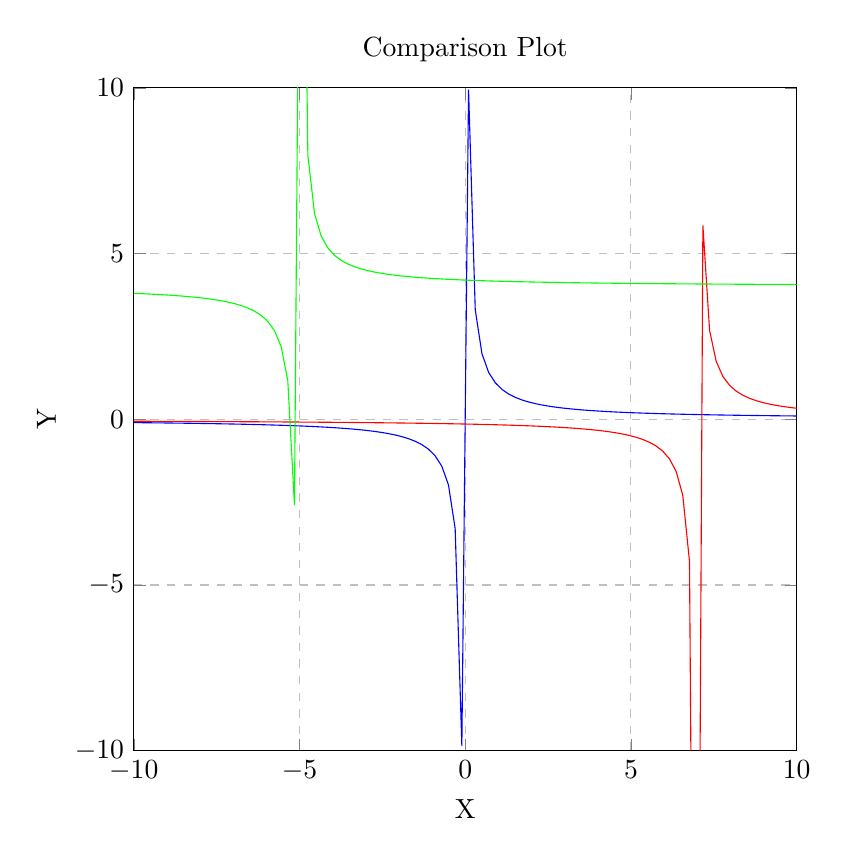
\begin{tikzpicture}
    \begin{axis} [
            title={Comparison Plot},
            xlabel={X},
            ylabel={Y},
            xmin=-10, xmax=10,
            ymin=-10, ymax=10,
            xtick={-10, -5, 0, 5, 10},
            ytick={-10, -5, 0, 5, 10},
            ymajorgrids=true,
            xmajorgrids=true,
            grid style=dashed,
        ]

        \addplot [
            domain=-10:10,
            samples=100,
            color=blue
        ]
        { 1/x };

        \addplot [
            domain=-10:10,
            samples=100,
            color=red
        ]
        { 1/(x-7) };

        \addplot [
            domain=-10:10,
            samples=100,
            color=green
        ]
        { 1/(x+5) + 4 };


    \end{axis}
\end{tikzpicture}


8) The function represented by the solid line is a transformation of the given function. Write an equation for the transformation \\
a) \(y = \left|x\right|\) \\
\hspace*{1em} 4 units to the right and 6 units down \\
\hspace*{1em} \(y = \left|x-4\right| - 6\) \\
b) \(y = \sqrt{x}\) \\
\hspace*{1em} 4 units to the left and 6 units up \\
\hspace*{1em} \(y = \sqrt{x+4} + 6\)


9) Give the graph of the  function \(y = f(x)\) sketch the graph of  \(y = f(x + 5)\) \\
\hspace*{1em} translate graph 5 units to the left


10) Give the graph of the  function \(y = f(x)\) sketch the graph of  \(y - 6 = f(x)\) \\
\hspace*{1em}  becomes \(y = f(x) + 6\)\\
\hspace*{1em} translate graph 6 units up


11) Give the graph of the  function \(y = f(x)\) sketch the graph of  \(y = f(x-3) + 2\) \\
\hspace*{1em} translate graph 3 untis to the right and 2 units up

\textbf{Quiz Stuff:} \\
Question 3: Determine the domain and range of the function \(y = \frac{1}{x-2}\) \\
my answer: \(D: x \neq 2 \And R: y  \in \mathbb{R} \) \\
correct answer: \(D: x \neq 2 \And R: y  \neq 0 \) \\
- this is reciprocal function so both \(y \neq 0 \And y \in \mathbb{R} \) but here the \(y  \neq 0 \) is correct


Question 3: if \((a, b)\) is a point on the graph \(y = f(x)\) dethermine a point on the graph of \(y = f(x - 2) + 3\) \\
my answer: \((a - 2, b + 3) \) \\
correct answer: \((a + 2, b + 3) \) \\
- \(y = f(x - 2) + 3\) is a translation of 2 units to the right and 3 units up so the a value is + 2 \\
\textbf{THIS IS SUPER CONFUSING SO MAKE SURE YOU WALK THROUGH THIS TRANSLATION WHEN ANSWERING THESE QUESTIONS}



\clearpage

\subsection{REFLECTING GRAPHS OF FUNCTIONS}


\textbf{Comparing \(y = \sqrt{x}\) to \(y = \sqrt{-x}\)}:


\(y = \sqrt{x}\) Base Points \\
\begin{tabular}{|c|c|}
    \hline
    x     & y     \\
    \hline
    x = 0 & y = 0 \\
    x = 1 & y = 1 \\
    x = 4 & y = 2 \\
    x = 9 & y = 3 \\
    \hline
\end{tabular}


\(y = \sqrt{-x}\) \\
- you can not take the square root of a negative number \(\therefore x \neq \) a positive number \\
- \(x\) can only be negative numbers and zero \\
\begin{tabular}{|c|c|}
    \hline
    x      & y     \\
    \hline
    x = 0  & y = 0 \\
    x = -1 & y = 1 \\
    x = -4 & y = 2 \\
    x = -9 & y = 3 \\
    \hline
\end{tabular}


\begin{tikzpicture}
    \begin{axis} [
            title={Comparison Plot},
            xlabel={X},
            ylabel={Y},
            xmin=-10, xmax=10,
            ymin=-10, ymax=10,
            xtick={-10, -5, 0, 5, 10},
            ytick={-10, -5, 0, 5, 10},
            ymajorgrids=true,
            xmajorgrids=true,
            grid style=dashed,
        ]

        \addplot [
            domain=0:9,
            samples=100,
            color=blue
        ]
        { sqrt(x) };

        \addplot [
            domain=0:-9,
            samples=100,
            color=red
        ]
        { sqrt(-x) };

    \end{axis}
\end{tikzpicture}


Desribe the effect of the graph when \(y = \sqrt{x}\) is replaced by \(y = \sqrt{-x}\): \\
- the graph is reflected in the \(y\) axis \\
- the point \((0,0)\) has a special name, it's called an \textbf{INVARIANT} point \\
- \textbf{INVARIANT POINT: A point that is unchanged by a transformation}
\clearpage


\textbf{Comparing \(y = \sqrt{x}\) to \(-y = \sqrt{x}\)}:


\(y = \sqrt{x}\) Base Points \\
\begin{tabular}{|c|c|}
    \hline
    x     & y     \\
    \hline
    x = 0 & y = 0 \\
    x = 1 & y = 1 \\
    x = 4 & y = 2 \\
    x = 9 & y = 3 \\
    \hline
\end{tabular}


\(y = \sqrt{-x}\) \\
IMPORTANT: Solve for \(y\) first \\
\hspace*{1em} \(-y = \sqrt{x}\) \\
\hspace*{1em} \(\frac{-y}{-1} = \frac{\sqrt{x}}{-1}\) \\
\hspace*{1em} \(y = -\sqrt{x}\) \\
\hspace*{1em} \(y = -\sqrt{1}\) \\
\hspace*{1em} \(y = -1\) \\
\begin{tabular}{|c|c|}
    \hline
    x     & y      \\
    \hline
    x = 0 & y = 0  \\
    x = 1 & y = -1 \\
    x = 4 & y = -2 \\
    x = 9 & y = -3 \\
    \hline
\end{tabular}


\begin{tikzpicture}
    \begin{axis} [
            title={Comparison Plot},
            xlabel={X},
            ylabel={Y},
            xmin=-10, xmax=10,
            ymin=-10, ymax=10,
            xtick={-10, -5, 0, 5, 10},
            ytick={-10, -5, 0, 5, 10},
            ymajorgrids=true,
            xmajorgrids=true,
            grid style=dashed,
        ]

        \addplot [
            domain=0:9,
            samples=100,
            color=blue
        ]
        { sqrt(x) };

        \addplot [
            domain=0:9,
            samples=100,
            color=red
        ]
        { -(sqrt(x)) };

    \end{axis}
\end{tikzpicture}

Desribe the effect of the graph when \(y = \sqrt{x}\) is replaced by \(-y = \sqrt{x}\) : \\
- the graph is reflected in the \(x\) axis \\
- \(-y = \sqrt{x}\) is the same as \(y = -\sqrt{x}\) \\
- this reflection also has an invariant point at (0,0)
\clearpage

\textbf{Comparing \(y = f(x)\) to \(x = f(y)\)}: \\
\(x = f(y)\) this is the \textbf{INVERSE} of \(y = f(x)\) \\
Graph the linear function \(y = 3x-1\) (Slope intercept form) \\
\(-1\) is the y intercept and the \(\frac{rise}{run}\) is \(\frac{3}{1}\) \\
slope is +ve so line goes from lower left to upper right \\
Graph the inverse function \(x = 3y-1\) (swap x and y) \\
Solve for \(y\) \\
\(x+1 = 3y\) \\
\(\frac{x}{3} + \frac{1}{3}=\frac{3y}{3}\) \\
\(y =\frac{1}{3}x + \frac{1}{3}\)


\begin{tikzpicture}
    \begin{axis} [
            title={Comparison Plot},
            xlabel={X},
            ylabel={Y},
            xmin=-10, xmax=10,
            ymin=-10, ymax=10,
            xtick={-10, -5, 0, 5, 10},
            ytick={-10, -5, 0, 5, 10},
            ymajorgrids=true,
            xmajorgrids=true,
            grid style=dashed,
        ]

        \addplot [
            domain=-10:10,
            samples=100,
            color=blue
        ]
        { 3*x-1 };

        \addplot [
            domain=-10:10,
            samples=100,
            color=red
        ]
        { 1/3 * x + 1/3 };

    \end{axis}
\end{tikzpicture}


Desribe the effect of the graph when \(y = 3x-1\) when x and y are switched : \\
- switching x and y describes a REFLECTION in the line \(y = x\) \\
\textbf{NOTE:} \(y = f^{-1}(x)\) is sometimes used to represent the the equation of the inverse \\
\(f^{-1}\) is NOT a negative exponent, it simply means the inverse


- reflecting points in this Comparison \\
- the inverse is not a function, it's a relation, not a function \\
- you can use the method of reflecting base points on the line y = x to graph the inverse but it is not
- to graph the inverse use the method of switch x, y


\begin{tabular}{|c|c|}
    \hline
    $y = f(x)$ & $y = f^{-1}(x)$ \\
    \hline
    (-3, 9)    & (9, -3)         \\
    (-4, 4)    & (4, -4)         \\
    (-6, 0)    & (0, -6)         \\
    (-8, 4)    & (4, -8)         \\
    (-9, 9)    & (9, -9)         \\
    \hline
\end{tabular}


\begin{tikzpicture}
    \begin{axis} [
            title={Comparison Plot},
            xlabel={X},
            ylabel={Y},
            xmin=-10, xmax=10,
            ymin=-10, ymax=10,
            xtick={-10, -5, 0, 5, 10},
            ytick={-10, -5, 0, 5, 10},
            ymajorgrids=true,
            xmajorgrids=true,
            grid style=dashed,
        ]

        \addplot coordinates
            { (-3, 9) (-4, 4) (-6, 0) (-8, 4) (-9, 9)};

        \addplot coordinates
            { (9, -3) (4, -4) (0, -6) (4, -8) (9, -9) };

    \end{axis}
\end{tikzpicture}


\textbf{Examples: } \\
1) Graph the function \(y=-\sqrt{x+2}+1\) \\
- this is a reflection on the x axis \\
- solve for y \\
Steps from solution: \\
Step 1) dethermine the base equation and then graph the base function \\
the base equation is \(y=\sqrt{x}\) \\
Step 2) Identify the transformations of the function \\
the -ve value out the fucntion indicates a reflection on the x axis \\
the x+2 indicates a shift of 2 units to the left \\
the -1 indicates a shift of 1 unit down

\begin{tabular}{|c|c|}
    \hline
    x  & y  \\
    \hline
    0  & -2 \\
    2  & -3 \\
    7  & -4 \\
    14 & -5 \\
    \hline
\end{tabular}


\begin{tikzpicture}
    \begin{axis} [
            title={Comparison Plot},
            xlabel={X},
            ylabel={Y},
            xmin=-10, xmax=10,
            ymin=-10, ymax=10,
            xtick={-10, -5, 0, 5, 10},
            ytick={-10, -5, 0, 5, 10},
            ymajorgrids=true,
            xmajorgrids=true,
            grid style=dashed,
        ]

        \addplot [
            domain=-10:10,
            samples=100,
            color=blue
        ]
        { (sqrt(x)) };

        \addplot [
            domain=-10:10,
            samples=100,
            color=red
        ]
        { -(sqrt(x+2)) - 1 };

    \end{axis}
\end{tikzpicture}


2) Graph the function \(f(x)=2x-4\) then sketch the graph of \(y = f^{-1}(x)\) (the inverse) \\
You should identify the function as a linear function \\
The graph is a straight line \\
To graph locate the y intercept (-4) and the slope (2) \\
so rise/run is \(\frac{2}{1}\) \\
draw the slope from the y intercept \\
Now that you have the graph drawn choose base points \\
Then switch the x and y values


\begin{tikzpicture}
    \begin{axis} [
            title={Comparison Plot},
            xlabel={X},
            ylabel={Y},
            xmin=-10, xmax=10,
            ymin=-10, ymax=10,
            xtick={-10, -5, 0, 5, 10},
            ytick={-10, -5, 0, 5, 10},
            ymajorgrids=true,
            xmajorgrids=true,
            grid style=dashed,
        ]

        \addplot [
            domain=-10:10,
            samples=100,
            color=blue
        ]
        { 2*x-4 };

        \addplot [
            domain=-10:10,
            samples=100,
            color=red
        ]
        { 1/2*x+2};

    \end{axis}
\end{tikzpicture}
\clearpage


3) Determine \(y = f^{-1}(x)\) the inverse of \(f(x)=\frac{1}{x-2}\) \\
\(y=\frac{1}{x-2}\) so the inverse is \(x=\frac{1}{y-2}\) \\
solve for y \\
multiply each side by the common denominator \(y-2\) \\
\((y-2)x=\frac{1}{y-2}(y-2)\) \\
Cancel the \(y-2\) \\
\((y-2)x=1\) \\
Divide both sides by x \\
\(\frac{(y-2)x}{x}=\frac{1}{x}\) \\
cancel the x's \\
\(y-2=\frac{1}{x}\) \\
\(y=\frac{1}{x} + 2\)

4) Given the graph of the function \(y = f(x)\) below, graph \(y = -f(x)\) \\
\(y = -f(x)\) indicates a reflection on the x axis \\
base points of the original function are \\
\begin{tabular}{|c|c|}
    \hline
    x  & y  \\
    \hline
    -7 & 0  \\
    -4 & 3  \\
    3  & -3 \\
    6  & 7  \\
    \hline
\end{tabular} \\
x values remain constant and y values are inverted \\
\begin{tabular}{|c|c|}
    \hline
    x  & y  \\
    \hline
    -7 & 0  \\
    -4 & -3 \\
    3  & 3  \\
    6  & -7 \\
    \hline
\end{tabular}


5) Given the graph of the function \(y = f(x)\) below, graph \(y = f(-x)\) \\
\(y = f(-x)\) indicates a reflection on the y axis \\
\begin{tabular}{|c|c|}
    \hline
    x  & y  \\
    \hline
    -7 & 0  \\
    -4 & 3  \\
    3  & -3 \\
    6  & 7  \\
    \hline
\end{tabular} \\
y values remain constant and x values are inverted \\
\begin{tabular}{|c|c|}
    \hline
    x  & y  \\
    \hline
    7  & 0  \\
    4  & 3  \\
    -3 & -3 \\
    -6 & 7  \\
    \hline
\end{tabular}


6) Given the graph of the function \(y = f(x)\) below, graph \(y = f^{-1}(x)\) \\
\(y = f^{-1}(x)\) indicates an inverse function\\
\begin{tabular}{|c|c|}
    \hline
    x  & y  \\
    \hline
    -7 & 0  \\
    -4 & 3  \\
    3  & -3 \\
    6  & 7  \\
    \hline
\end{tabular} \\
invert the x and y values \\
\begin{tabular}{|c|c|}
    \hline
    x  & y  \\
    \hline
    0  & -7 \\
    3  & -4 \\
    -3 & 3  \\
    7  & 6  \\
    \hline
\end{tabular}
\clearpage


7) If the point \((-3, 2)\) is on the graph of the function \(y = f(x)\) determine the new coordinates of the image of this point on the function \\
a) \(y = f(-x)\) \\
reflection on the y axis, x value is inverted so \((3, 2)\) \\
b) \(y = -f(x)\) \\
reflection on the x axis, y value is inverted so \((-3, -2)\) \\
c) \(y = f^{-1}(x)\) \\
inversion, x and y value is inverted so \((2, -3)\)


formative Assessment relflecting graphs of functions



\end{document}
